\subsection{Executor Clusters}\label{subsec:archexecutors}

The executor clusters are a set of cluster and each cluster is composed of a set
of Erlang processes. The choice for which it was decided to implement a cluster
structure will be described in \secref{subsec:archtolerance}. Each executor
cluster manages a subset of auctions of the system (the assignment of an auction
to a cluster is decided, as previously mentioned, by the dispatchers). Each
cluster communicates with Mnesia (we will see later) for the data persistence
and manages the progress of the auctions for which it is responsible. In
particular, for each auction, the cluster must calculate the so-called
\textbf{AuctionState}, \idest*{produce the list of current winning bids each
time a bid is added or deleted}.


Following the \underline{all-or-nothing} semantics described in the
specifications, the \code{AuctionState} is calculated,trying to maximize the profit 
for the Agent, by taking the bids with the highest value (for the same value, 
the oldest bid is considered as the best) and that the sum of the quantities of items 
requested by these is less than or equal to the quantity of items for sale. 
Furthermore, it is ensured that only one bid per user is among the winning ones.

\figref{fig:auction_state_example} shows an \code{AuctionState} computation
example.

\begin{figure}[htb]
	\centering
	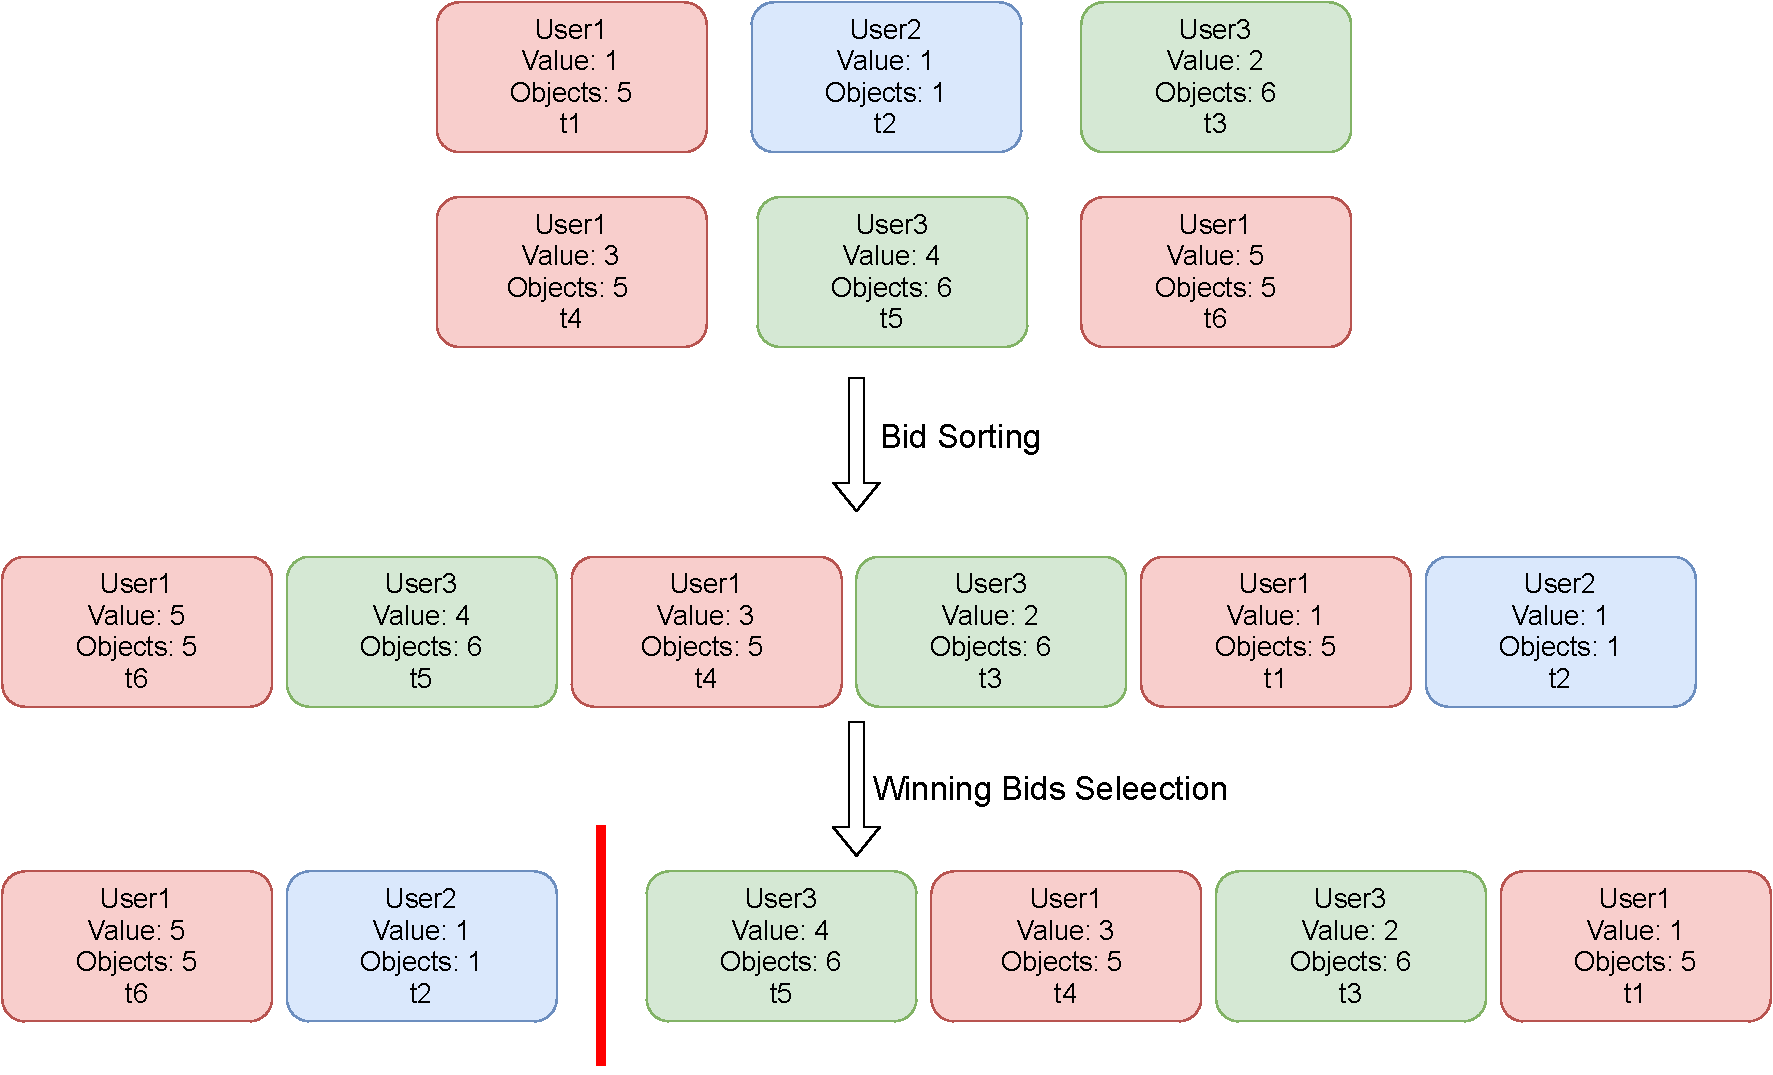
\includegraphics[width=\textwidth]{auction_state_example}
	\caption{AuctionState Computation}\label{fig:auction_state_example}
\end{figure}

The \code{AuctionState} is kept in memory in order to be sent upon request by
the application server and is recalculated (and subsequently sent) every time an
offer is added or deleted. Executor processes are implemented through the
\textit{gen\_server} behavior.
